% Template for ICASSP-2021 paper; to be used with:
%          spconf.sty  - ICASSP/ICIP LaTeX style file, and
%          IEEEbib.bst - IEEE bibliography style file.
% --------------------------------------------------------------------------
\documentclass{article}
\usepackage{spconf,amsmath,graphicx}
\usepackage{hyperref}
\graphicspath{ {./images/} } % set path to images

% Example definitions.
% --------------------
\def\x{{\mathbf x}}
\def\L{{\cal L}}

% Title.
% ------
\title{Fine-tuning MLLM for multimodal question answering}
%
% Single address.
% ---------------
\name{Sara Boukili \qquad Philippe Gélinas \qquad Antoine Reid}
%
% For example:
% ------------
\address{Université Laval\\
	Département d'informatique et de génie logiciel\\
	IFT-4030 Apprentissage automatique pour le traitement du signal}

\begin{document}
%\ninept
%
\maketitle
%
\begin{abstract}
The abstract should appear at the top of the left-hand column of text, about
0.5 inch (12 mm) below the title area and no more than 3.125 inches (80 mm) in
length.  Leave a 0.5 inch (12 mm) space between the end of the abstract and the
beginning of the main text.  The abstract should contain about 100 to 150
words, and should be identical to the abstract text submitted electronically
along with the paper cover sheet.  All manuscripts must be in English, printed
in black ink.
\end{abstract}
%
\begin{keywords}
One, two, three, four, five
\end{keywords}
%
\section{Introduction}
\label{sec:intro}
LLM fine-tuning is a very active research topic and new methods are constantly being proposed. However, fine-tuning LLMs is computationaly expensive and most current techniques are prohibitively expensive for consumer hardware. We aim to fine-tune a multimodal LLM (MLLM) for a multiple-choice question answering task with consumer-grade hardware. Therefore, we limit ourselves to GPUs with no more than 15GB of VRAM and LLMs with no more than 8b parameters. We use the ScienceQA dataset as a benchmark to evaluate different fine-tuning techniques and models. We focus mainly on parameter-efficient fine-tuning as they allow training on consumer hardware. We also explored prompt-tuning which can be an alternative to fine-tuning. We briefly explored using RAG instead of fine-tuning but found this method to be unsuitable for our task. We further investigated prompt-tuning as another fine-tuning method, which achieves task-specific adaptation by merely using model prompts without modifying model weights. This approach aligns with our hardware resources while maintaining strong task-specific performance.

\section{Literature review}
\label{sec:litreview}

LoRA (Low-Rank Adaptation) is a fine-tuning technique for LLMs introduced by \cite{lora}. It deviates from regular fine-tuning by freezing the original model weights and by updating a separate set of weights which are then added to the original weights. In regular fine-tuning an entire weight update matrix ($\Delta W$) is combined with the pre-trained weights. LoRA separates $\Delta W$ into 2 low-rank matrices that approximate it. This method significantly reduces the number of trainable parameters. Along with the reduced computational load this brings, it can also help prevent overfitting. Compared to other adapter based fine-tuning techniques, LoRA does not introduce increased inference latency during inference. The downside of LoRA is that it introduces a new hyperparameter, $r$, which must be optimized. This hyperparameter represents the inner dimension of the low-rank matrices.\par

QLoRA \cite{qlora} is a modification of LoRA that introduces increased memory efficiency due to storing weight parameters with 4-bit precision. To achieve this, the authors used 3 concepts : a new data type, 4-bit NormalFloat, which is theoretically optimal for normally distributed data, double quantization of quantization constants to increase the memory efficiency, and paged optimizers to handle memory spikes. \cite{qlora} observed performance levels similar to those of LoRA. Another LoRa variant is DoRA \cite{dora}, which is supposed to outperform LoRa for fine-tuning LLMs for various tasks, including ours, which relates to image-text understanding. DoRA decomposes the weights of a pre-trained model into magnitude and direction components. DoRA can be applied in the same way as LoRA, and allows its variants like QDoRA.\par

ProMoT (Prompt Tuning with Model Tuning) \cite{valizadehaslani2022twostagefinetuningnovelstrategy} addresses the challenge of language models becoming overly specialized during fine-tuning, which can reduce their general capabilities. It uses a two-stage approach that offloads format learning to additional parameters through prompt tuning, allowing for comparable performance on the fine-tuned task while preserving or even enhancing general in-context learning abilities. This flexibility in managing various output formats and task types is particularly beneficial for the diverse question types in the ScienceQA dataset.\par

An extensive review of RAG \cite{ragreview} has found that RAGs can help address hallucination and outdated knowledge problems. The advantage of RAG is that they allow for continuous knowledge update to the model and can allow an LLM to incorporate knowledge outside of the training domain. RAG are not always better than fine-tuning, especially for tasks which require specific data formats as inputs and a response in a particular style.\par



\section{Method}
\label{sec:method}

\subsection{Parameter-Efficient Fine-Tuning (PEFT)}
For this section, we will test PEFT methods on two models: LLaVA-1.5\cite{liu2023llava} and Idefics2\cite{idefics2}. These
two models were chosen because they possess a number of parameters small enough to be suitable for training on consumer-grade GPUs, while still being able to handle multimodal inputs (image and text) which is required for the task at hand. Idefics2 contains roughly 8b parameters while LLaVA-1.5 contains roughly 7b parameters. Idefics2 was created by the HuggingFace team and was shown to outperform much larger LLMs on several benchmarks. LLaVA-1.5 uses CLIP ViT-L/14 as a visual encoder and Vicuna (itself based on Llama) as the LLM decoder. During fine-tuning we keep the vision encoder (the part of the model that tokenizes the images) frozen.\par

Traditional fine-tuning is far too costly for consumer hardware because of the sheer numer of parameters to train. For example, Idefics2 contains roughly 8.4 billion parameters, which would require about 16GB of VRAM to store. When fine-tuning with Adam optimizer, this would be even greater because the optimizer stores 3 copies of the weights. PEFT methods make fine-tuning larger NLP models much more accessible by only training a small subset of model parameters while keeping the vast majority of the base model's parameters frozen.\par

LoRA significantly reduces the number of trainable parameters by approximating a weight update matrix with two low-rank matrices. LoRA only applies to linear layers of the model. LoRA can reduce the number of trainable parameters by 10,000 times. When using LoRA fine-tuning with a rank of 8 for Idefics2, we reduced the number of trainable parameters from 8.4b to 23.3m. We are training less than 0.1\,\% of the total model parameters! LoRA methods introduce two hyperparameters to set: the rank of the adapter matrices $r$ and the layers which are actually fine-tuned.\par

Despite the important reduction in trainable parameters LoRA offers, it can still be too costly to fine-tune an LLM with 8b parameters on a consumer GPU. This is because the base model, even when frozen, requires too much storage space. To alleviate this problem, we utilize quantization. Generally, the model parameters of an LLM are stored in 16 or 32-bit formats. Quantization compresses these parameters into 4-bit which significantly reduces the memory footprint. Although quantization introduces a loss of information, the impact of the quantization error is minimized by the fine-tuning (during training the model learns and incorporates the quantization error). QLoRA combines quantization and LoRA and is the first PEFT method we will use. It is important to understand that only the frozen parameters are stored in 4-bit, the LoRA adapter layers and the Adam optimizer are not quantized.\par

LoRA was found to have much a much different learning behavior than full fine-tuning. Furthermore, LoRA performs worse than full fine-tuning in certain situations. DoRA corrects these shortcomings by decomposing the pretrained weights into their magnitude and direction. LoRA is then applied to the directional component, while the magnitude component is trained as is. DoRA has a greater memory overhead than LoRA since there are more trainable parameters. The second PEFT method we utilize is a quantized version of DoRA.\par

We will fine-tune both models with PEFT methods on a train set of the ScienceQA dataset and then evaluate the performance of the model on the test set. Given that there are a varying number of choices (between 2 and 5), we use accuracy as a performance metric.

\subsection{Prompt tuning}

We adopted a prompt-tuning approach inspired by ProMot, using structured prompts to guide the model in answering multiple-choice ScienceQA tasks. Our prompts included contextual hints and lectures if available, with questions and choices formatted for clarity. The tokenization was performed with DeBERTa-base tokenizer, and a transformer-based encoder was fine-tuned to align with this structured input. 

\subsubsection{Model: DeBERTa}

As said before, we used DeBERTa (Decoding-enhanced BERT with Disentangled Attention) model as the backbone for our prompt-tuning experiments. This model improves upon its predecessors, BERT and RoBERTa, by introducing disentangled attention mechanisms and an enhanced mask decoder. This architecture allows for better contextual understanding and improved performance across a range of Natural Language Understanding tasks, particularly on datasets with a variety of input formats the one we're working with ScienceQA. \\
We chose DeBERTa due to its state-of-the-art performance on multiple NLU benchmarks and its ability to efficiently handle diverse linguistic patterns. With over 80GB of training data, the model is well-suited for our objective of answering multimodal, multiple-choice science questions.

\subsubsection{Prompt Structure:}

One of the key innovations in our approach was the design of structured prompts used especially for the ScienceQA dataset. Each prompt guides the model in reasoning through the questions and available contextual information, such as hints or lectures. \\
The structure of the prompt was carefully crafted to include:
\begin{itemize}
    \item Role Assignment: Defining the model's role as a specialized science tutor.
    \item Contextual Information: Incorporating lecture content and hints, if available.
    \item Question Presentation: Clearly stating the question and listing the multiple-choice options.
    \item Task Instruction: Directing the model to provide the most accurate answer based on logical reasoning and scientific principles.
\end{itemize}

\begin{figure}
  \centerline{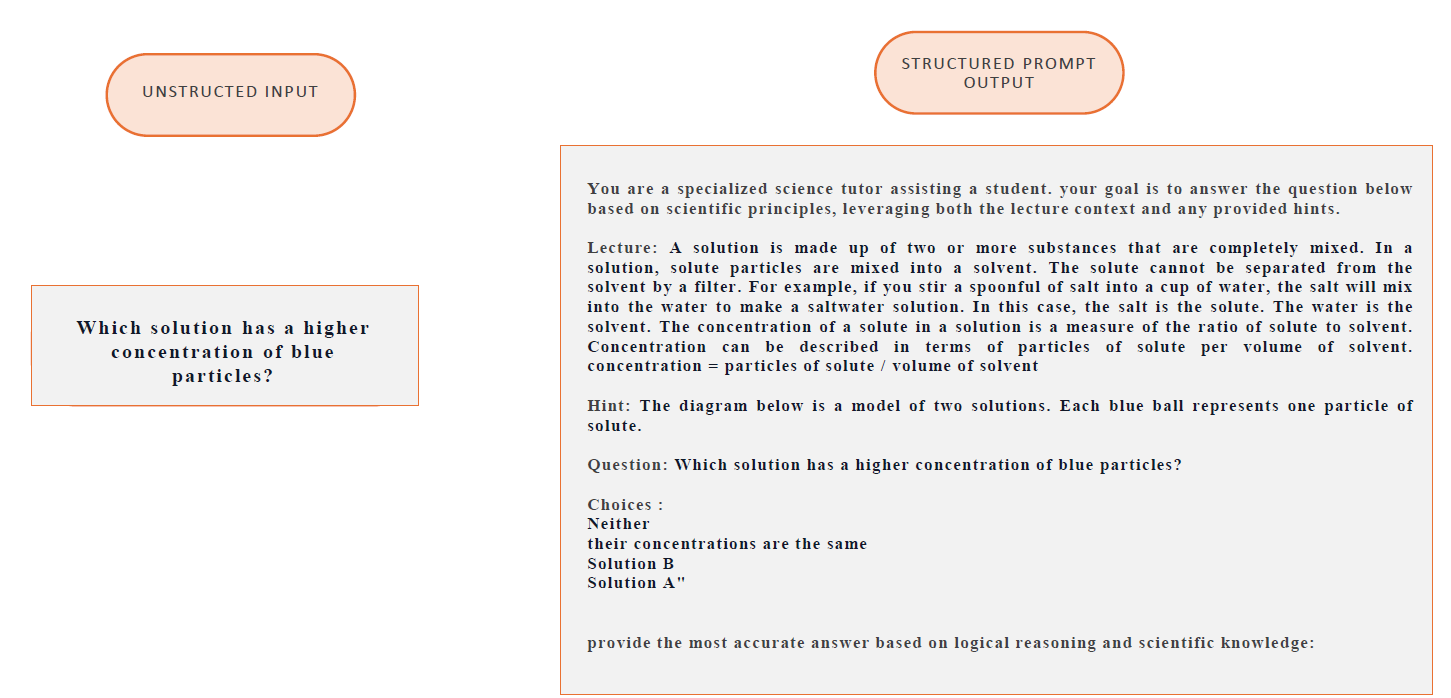
\includegraphics[scale=0.2]{rapport/images/prompt.png}}
  \caption{Example of an unstructured and a structured prompt from the ScienceQA dataset}
  \label{fig:example_prompt}
\end{figure}


\begin{table*}[t]
  \centering
  \begin{tabular}{lrrr}
    \hline
    Model & Trainable parameters & Training time & Accuracy (\%)\\ 
    \hline
    Idefics2 QLoRA (r=8) & 23,326,720 & 6h 18min & 89.14\\ 
    Idefics2 QLoRA (r=4) & 11,663,360 & 4h 52min & 88.20\\ 
    Idefics2 QLoRA last 50 layers (r=8) & 4,734,976 & 1h & 77.00\\
    Idefics2 QDoRA (r=6) & 19,033,856 & 10h 13min & 89.54\\
    LLaVA QLoRA (r=6) & 15,876,096 & 10h 20min & 83.28\\
    LLaVA QDoRA (r=5) & 14,663,680 & 14h 30min & 84.13\\
    Prompt-tuning & - & 4 days & 79.44\\
    \hline
  \end{tabular}
  \caption{Accuracy of models on test dataset}
  \label{tab:model_performance}
\end{table*}

\subsection{Retrieval-augmented generation (RAG)}
We briefly explored using RAG instead of fine-tuning but quickly ruled out this method. Inference with RAG is very long (it can take minutes to answer a single question) and creating a vector database centered around relevant scientific knowledge would've been too time consuming. Exploring RAG in more detail could be the subject of a future project.

\section{Experiments}
\label{sec:experiments}

\begin{figure}
  \centering
  \centerline{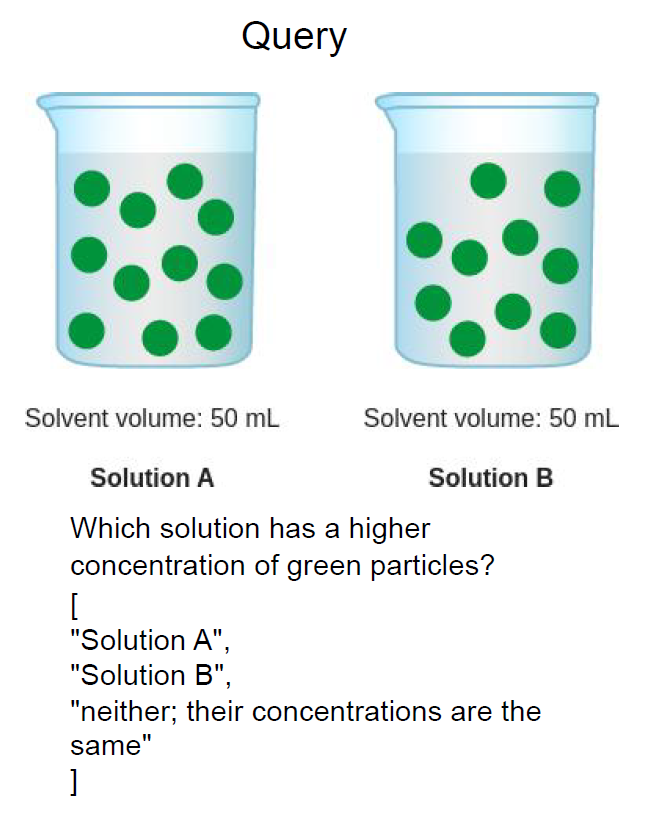
\includegraphics[scale=0.5]{example_question.png}}
  \caption{Example question from the ScienceQA dataset}
  \label{fig:example_q}
\end{figure}

\subsection{ScienceQA dataset}
As mentioned, we will use the ScienceQA dataset. The ScienceQA dataset contains 21\,208 multimodal multiple-choice questions collected from primary and high school curricula. The questions are separated into 3 subjects: natural science, language science, and social science. Roughly 49\,\% of the questions have an image context, 48\,\% have a text context, and 31\,\% have both. An interesting aspect of the ScienceQA dataset is that most question contain lectures (84\,\%) and detailed explanations (91\,\%) that help answer the question. The dataset has already been split into train, test, and validation sets on HuggingFace. The train set contains 12,726 observations, whereas the test and validation sets each contain 4,241 observations. Figure \ref{fig:example_q} shows a typical question from the dataset. We want the model to answer the question by returning the index of the list of choices corresponding to the correct answer. For example, in the question asked in figure \ref{fig:example_q}, the model should return "0".

\subsection{Training details}

We initially tried to have the pretrained models accomplish the task without fine-tuning in order to have a benchmark. However, this proved futile as without fine-tuning the models were unable to answer the questions in the desired format. In fact, they would often hallucinate and return answers unrelated to the question.

For PEFT methods, we trained within the HuggingFace environnement. Specifically, the PEFT package allows us to fine-tune HuggingFace models with LoRA and DoRA. We opted to use HuggingFace as it is very well documented and we can do everything we need, from data importation to computing test accuracy, with the same API. In order to have comparable training times, all fine-tuning was done on the same GPU. HuggingFace also allowed us to easily quantize the models.

The ScienceQA dataset required very little pre-processing. All that was required was to transform the answers from integers into strings since the models return a string.

We tried to vary the QLoRA hyperparameters to gauge their affect on performance. We tested Idefics2 with $r=4$ and $r=8$. We also applied QLoRA to only the last 50 linear layers of Idefics2. Since QDoRA has a greater memory requirement, we had to use a rank of 6 to be able to train on GPU. We did not explore the impact of varying hyperparameters with LLaVA because this model took much longer to train. We believe this is due to LLaVA taking much longer to perform the forward pass than Idefics2.

We only trained the models for 2 epochs as this was sufficient to obtain decent results and the training times were costly. We used the largest batch size we could during training but this was often a small value such as 2. To compensate, we added gradient accumulation steps to increase the effective batch size. Gradient accumulation delays the updating of model parameters by accumulating gradients over a certain number of batches. For example, with a batch size of 2 and 8 gradient accumulation steps, the effective batch size is 16. We use some weight decay to reduce overfitting. This is important since we have a relatively small dataset for deep learning. Finally we utilize a warm-up period at the beginning of training to avoid having giving increased importance to the initial observations. We used a warm-up period of roughly 5\,\% of the total training steps. Without a warm-up period, the model can skew badly towards the initial observations. Thus, it would require more training to converge as it "un-trains" early mistakes.

\subsection{Results}

Table \ref{tab:model_performance} presents the results of our various models and fine-tuning techniques.


Not suprisingly Idefics2 beats LLaVA-1.5 because it accepts greater image resolution and has beaten LLaVA-1.5 in other benchmarks.\cite{idefics2}

Even though, LLaVA QDoRA has less trainable parameters than LLaVA QLoRA (because they don't have
the same rank), it still managed to outperform the latter. This matches the claim that DoRA
is supposed to offer better performance than LoRA, although it requires more training time.

The same can be said about the Idefics2 results. The best performance of all the models is the one
by Idefics2 trained with QDoRA (r=6), even though it's not the model with the most trainable parameters. But again,
this comes with additional training time requirements.

Overall, the results are aligned with common sense reasoning. For each model, the more trainable parameters you have,
the better performance you get. The only exception is when you compare QLoRA and QDoRA. By separating the weights into
their magnitude and orientation components, as is the case in QDoRA, it seems the models are able
to augment their learning capacities compared to classic QLoRA fine-tuning. Although, QDoRA does come with
greater memory and time requirements.

Prompt-tuning offers an interesting alternative approach to other more conventional fine-tuning methods tested, but it seems
that the temporal costs are not worth the performance.



\section{Conclusion}
\label{sec:conclusion}

By employing parameter-efficient fine-tuning techniques like QLoRA and QDoRA, the feasibility of achieving high performance without the computational burden of full fine-tuning was validated. The experiments indicate that QDoRA outperforms QLoRA, even with less trainable parameters, albeit with increased memory and time requirements. Additionally, the Idefics2 model consistently outperformed LLaVA-1.5 across different configurations, reinforcing its suitability for multimodal question-answering tasks.

Prompt tuning was explored as another alternative to full fine-tuning, but its longer training times and relatively lower accuracy highlighted its limitations for this dataset. Concerning retrieval-augmented generation (RAG), it seems to be unsuitable due to inference latency and preparation overhead.

Future work could involve optimizing hyperparameters more comprehensively, evaluating newer PEFT techniques, or testing current methods more systematically across different rank values and choices of trainable layers.

% To start a new column (but not a new page) and help balance the last-page
% column length use \vfill\pagebreak.
% -------------------------------------------------------------------------
%\vfill
%\pagebreak


\vfill\pagebreak


% References should be produced using the bibtex program from suitable
% BiBTeX files (here: strings, refs, manuals). The IEEEbib.bst bibliography
% style file from IEEE produces unsorted bibliography list.
% -------------------------------------------------------------------------
\bibliographystyle{IEEEbib}
\bibliography{refs}

\section{Github}

The code can be accessed at : \url{https://github.com/dramatic-bat-flip/project_MLSP}

\end{document}
